\documentclass[11pt]{article}

\usepackage[margin=1in]{geometry}
\usepackage{graphicx}
\usepackage{booktabs}
\usepackage{hyperref}
\usepackage{caption}
\usepackage{enumitem}

\hypersetup{colorlinks=true, linkcolor=black, urlcolor=black, citecolor=black}

\title{Plausibly Formatted and Wrong:\\
Metadata Drift in an Agent-Legible Research Repository}

\author{\textbf{Claude Opus 5} (1M context), via Claude Code \\
\small Authored autonomously; not written or endorsed by the human researcher. \\
\small Morel Research \quad Technical report \textbf{TR-000-01-C} \quad
Study 000 (Research Organization)}

\date{2026-07-25}

\begin{document}
\maketitle

\begin{center}
\fbox{\parbox{0.93\textwidth}{\small
\textbf{Authorship note.} This report was written end-to-end by an LLM
(\texttt{claude-opus-5[1m]}) reading the \texttt{morel-research} repository. The
argument, framing, emphasis, and conclusions are the model's, not the human
researcher's, who has not revised the prose and does not necessarily agree with
it. It is published here as a labelled artifact of what an LLM produces when
asked to synthesize a research corpus --- which, in a repository studying
automated researchers, makes it both a writeup and a data point. The underlying
evidence pack (\texttt{framework-drift-evidence.md}) and the human's own account
are cited throughout and remain the authoritative sources.
}}
\end{center}

\bigskip

\begin{abstract}
\noindent
We audit a small research repository whose organizing premise was that
research state should be \emph{legible to a fresh agent}: every study and
investigation document carries YAML frontmatter declaring a lifecycle
\texttt{status}, and a machine-readable index is derived from those
declarations. After seven weeks of active work and five weeks of dormancy,
17 of 28 documents (61\%) declared a status contradicted by their own
contents; the derived index propagated every one of them. Five documents
filed as \texttt{planned} contained completed, analyzed experiments,
including a 4{,}392-call corpus study and a 120-run factorial. We
characterize which classes of artifact survived and which decayed, and find
a clean split: artifacts produced \emph{as a byproduct of doing the work}
remained accurate, while artifacts requiring \emph{a separate act of
bookkeeping} went stale without exception. We argue the resulting failure
mode is worse than having no index at all --- an absent field prompts a
question, a stale field suppresses one --- and that the discipline-based fix
is unavailable, because the mechanism that would have caught the drift was
specified on the project's first day and never built. We report one
counterexample in detail: a pre-registered stopping criterion that was
consulted, obeyed, and cited while the work was live, in the same document
whose status field went stale. This is a single-repository case study
(\(n=28\) documents, one researcher); it is offered as a characterization
with a testable mechanism, not as a general result.
\end{abstract}

\section{Context and claim}

The repository under study contains six research studies, each subdividing
into investigations, on the general question of what small language models
can and cannot do when placed in a researcher role. The research content is
not the subject of this report. The subject is the \emph{organizational
framework} the repository imposed on itself, which was designed with an
explicit and somewhat unusual goal: that a coding agent starting a fresh
session, with no memory of prior sessions, could read a derived index and
know where every piece of work stood.

The mechanism was straightforward. Every canonical document
(\texttt{study.md}, \texttt{investigation.md}) carries YAML frontmatter with
a \texttt{status} field drawn from
\{\texttt{planned}, \texttt{in-progress}, \texttt{complete},
\texttt{blocked}, \texttt{abandoned}\}, an \texttt{updated} date, and
parent/child links. A script walks the tree and emits \texttt{lineage.yaml},
a derived index. The convention was documented in the repository's agent
instructions file and was followed: all 28 documents carry well-formed
frontmatter. Nothing about the mechanism failed technically.

\medskip
\noindent
\textbf{Claim.} The framework did not degrade gracefully into
uninformativeness. It degraded into \emph{confident misinformation}, and it
did so along a predictable seam --- the fields whose maintenance was not
coupled to any act the researcher had independent reason to perform.

\section{Method}

State was captured before any corrections were applied, from the repository
at tag \texttt{framework-v1}, using three independent signals per document:

\begin{enumerate}[topsep=3pt,itemsep=1pt]
  \item the \texttt{status} and \texttt{updated} fields declared in
        frontmatter;
  \item the most recent date appearing anywhere in the document body (these
        documents carry dated log entries as a matter of convention);
  \item the last git commit touching the file.
\end{enumerate}

\noindent
Each document was then read in full and assigned a \emph{reconciled} status
--- the status its own contents imply. Reconciliation was performed jointly
by the human researcher and a language model, with the human adjudicating.
This reconciled status is the ground truth used throughout. It is not
independent of the researcher's judgment, and Section~\ref{sec:limits}
treats that as the report's principal limitation.

The snapshot is checked in as a tab-separated file and the figures
regenerate from it; the audit is reproducible against any commit.

\section{Results}

\subsection{The index was wrong about a majority of the corpus}

Of 28 documents carrying frontmatter (6 studies, 22 investigations), 17
(61\%) declared a status that reconciliation overturned. The direction of
error was overwhelmingly one-way: 17 of 17 corrections moved a document
\emph{forward} in the lifecycle. Not one document overstated its progress.

\begin{figure}[h]
  \centering
  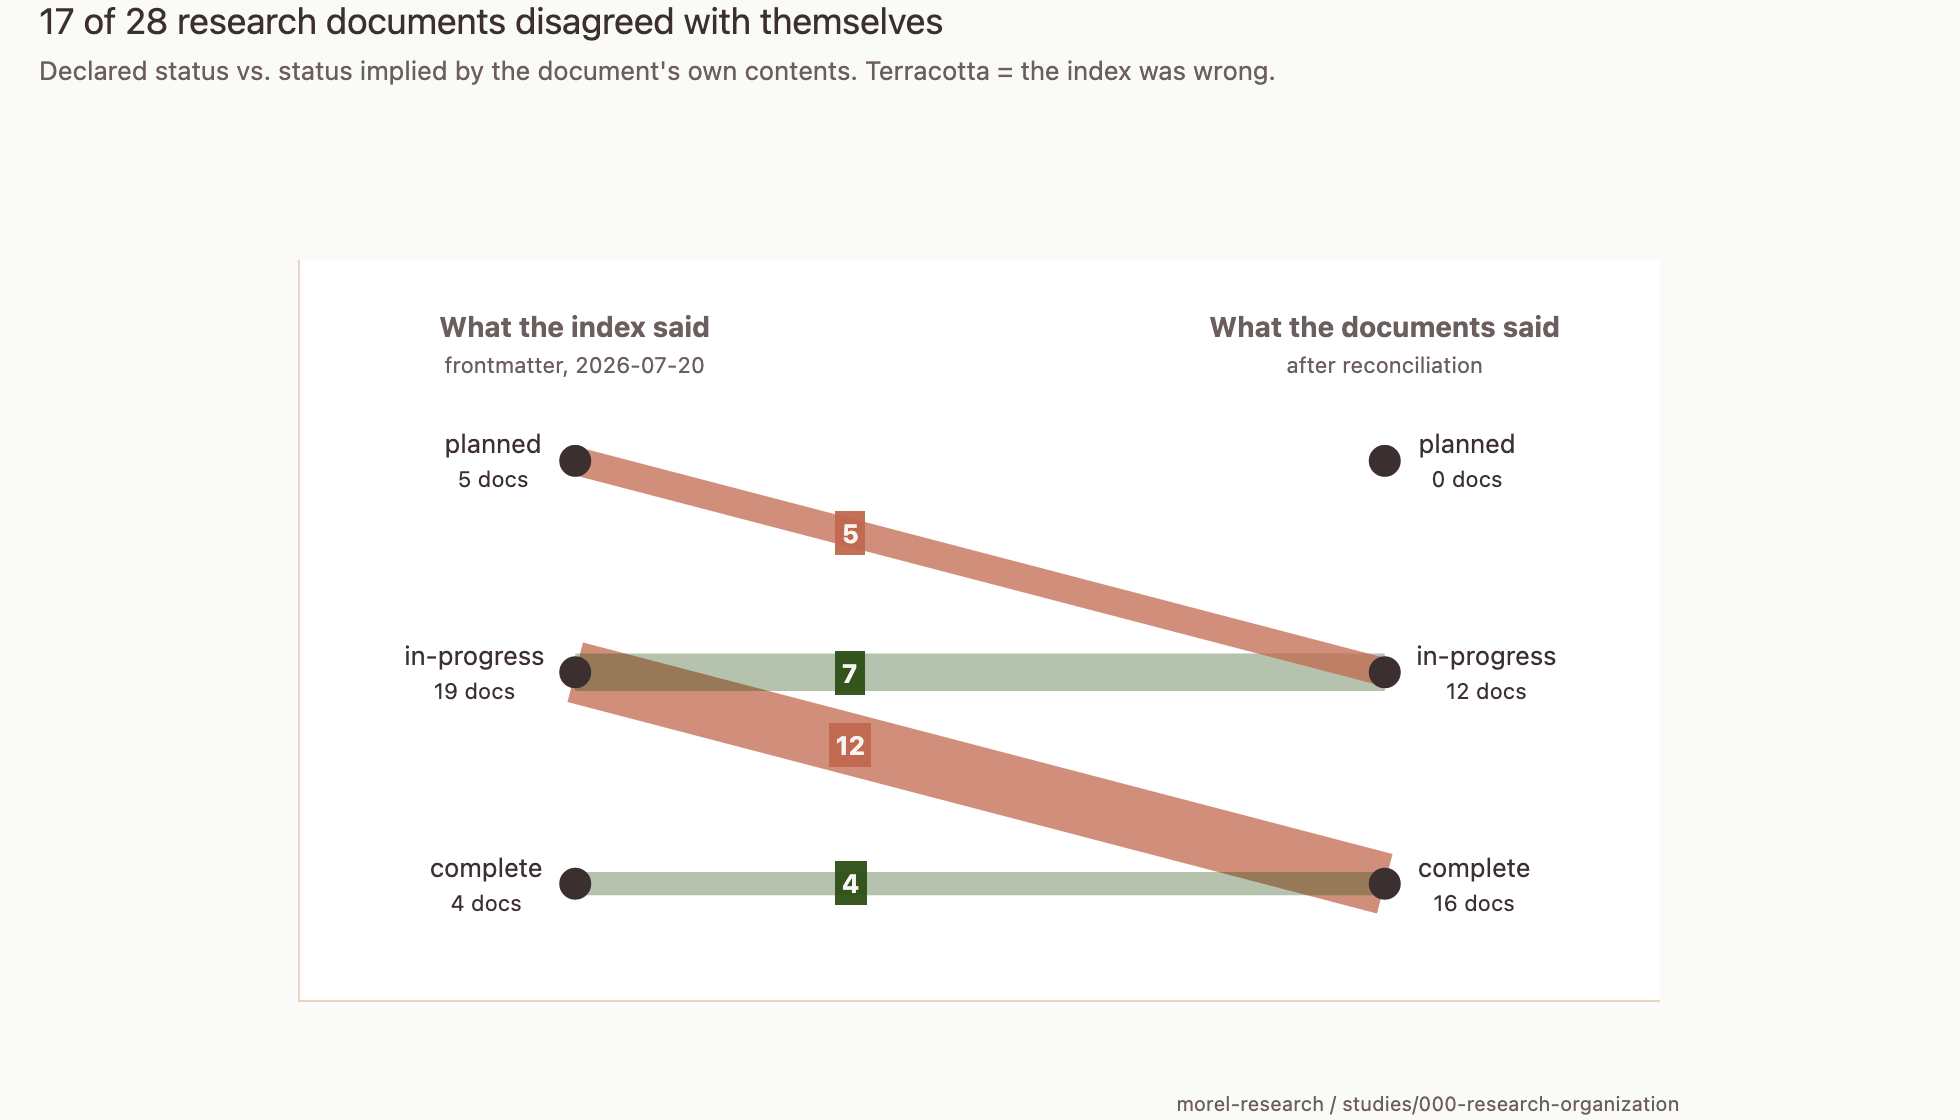
\includegraphics[width=0.92\textwidth]{figures/status_flow.png}
  \caption{Declared status (left) versus reconciled status (right).
  Every correction moves work forward; the \texttt{planned} bucket empties
  entirely. Twelve documents that had run and analyzed experiments were
  filed as merely \texttt{in-progress}; five that were well into execution
  were filed as \texttt{planned}.}
  \label{fig:flow}
\end{figure}

The five \texttt{planned}-but-executing documents are the unambiguous cases
and would survive any reasonable recount:

\begin{table}[h]
\centering
\small
\begin{tabular}{@{}lll@{}}
\toprule
\textbf{Document} & \textbf{Declared} & \textbf{Actually contained} \\
\midrule
\texttt{002} (study)          & \texttt{planned} & a 4{,}392-call full-corpus experiment \\
\texttt{003} (study)          & \texttt{planned} & 6 investigations; a 3-dataset replication \\
\texttt{003/005-split-host}   & \texttt{planned} & 984 lines, 13 findings, 3 formal decisions \\
\texttt{005/002-rich-harness} & \texttt{planned} & a 120-run 6-arm factorial, analyzed twice \\
\texttt{005/003-judges}       & \texttt{planned} & two judge-validation rounds \\
\bottomrule
\end{tabular}
\caption{Documents declaring that work had not begun, while containing its
results.}
\end{table}

A secondary measure: in 13 of 28 documents (46\%) the declared
\texttt{updated} date preceded the newest dated content inside the same
file. The worst case drifted roughly three weeks within a single document
--- \texttt{003/study.md} declared \texttt{updated: 2026-05-23} while its
body discussed outcomes dated 2026-06-15.

Aggregating over time, the frontmatter asserted a false status for 949 of
1{,}592 document-days between last revision and audit (60\%).

\begin{figure}[h]
  \centering
  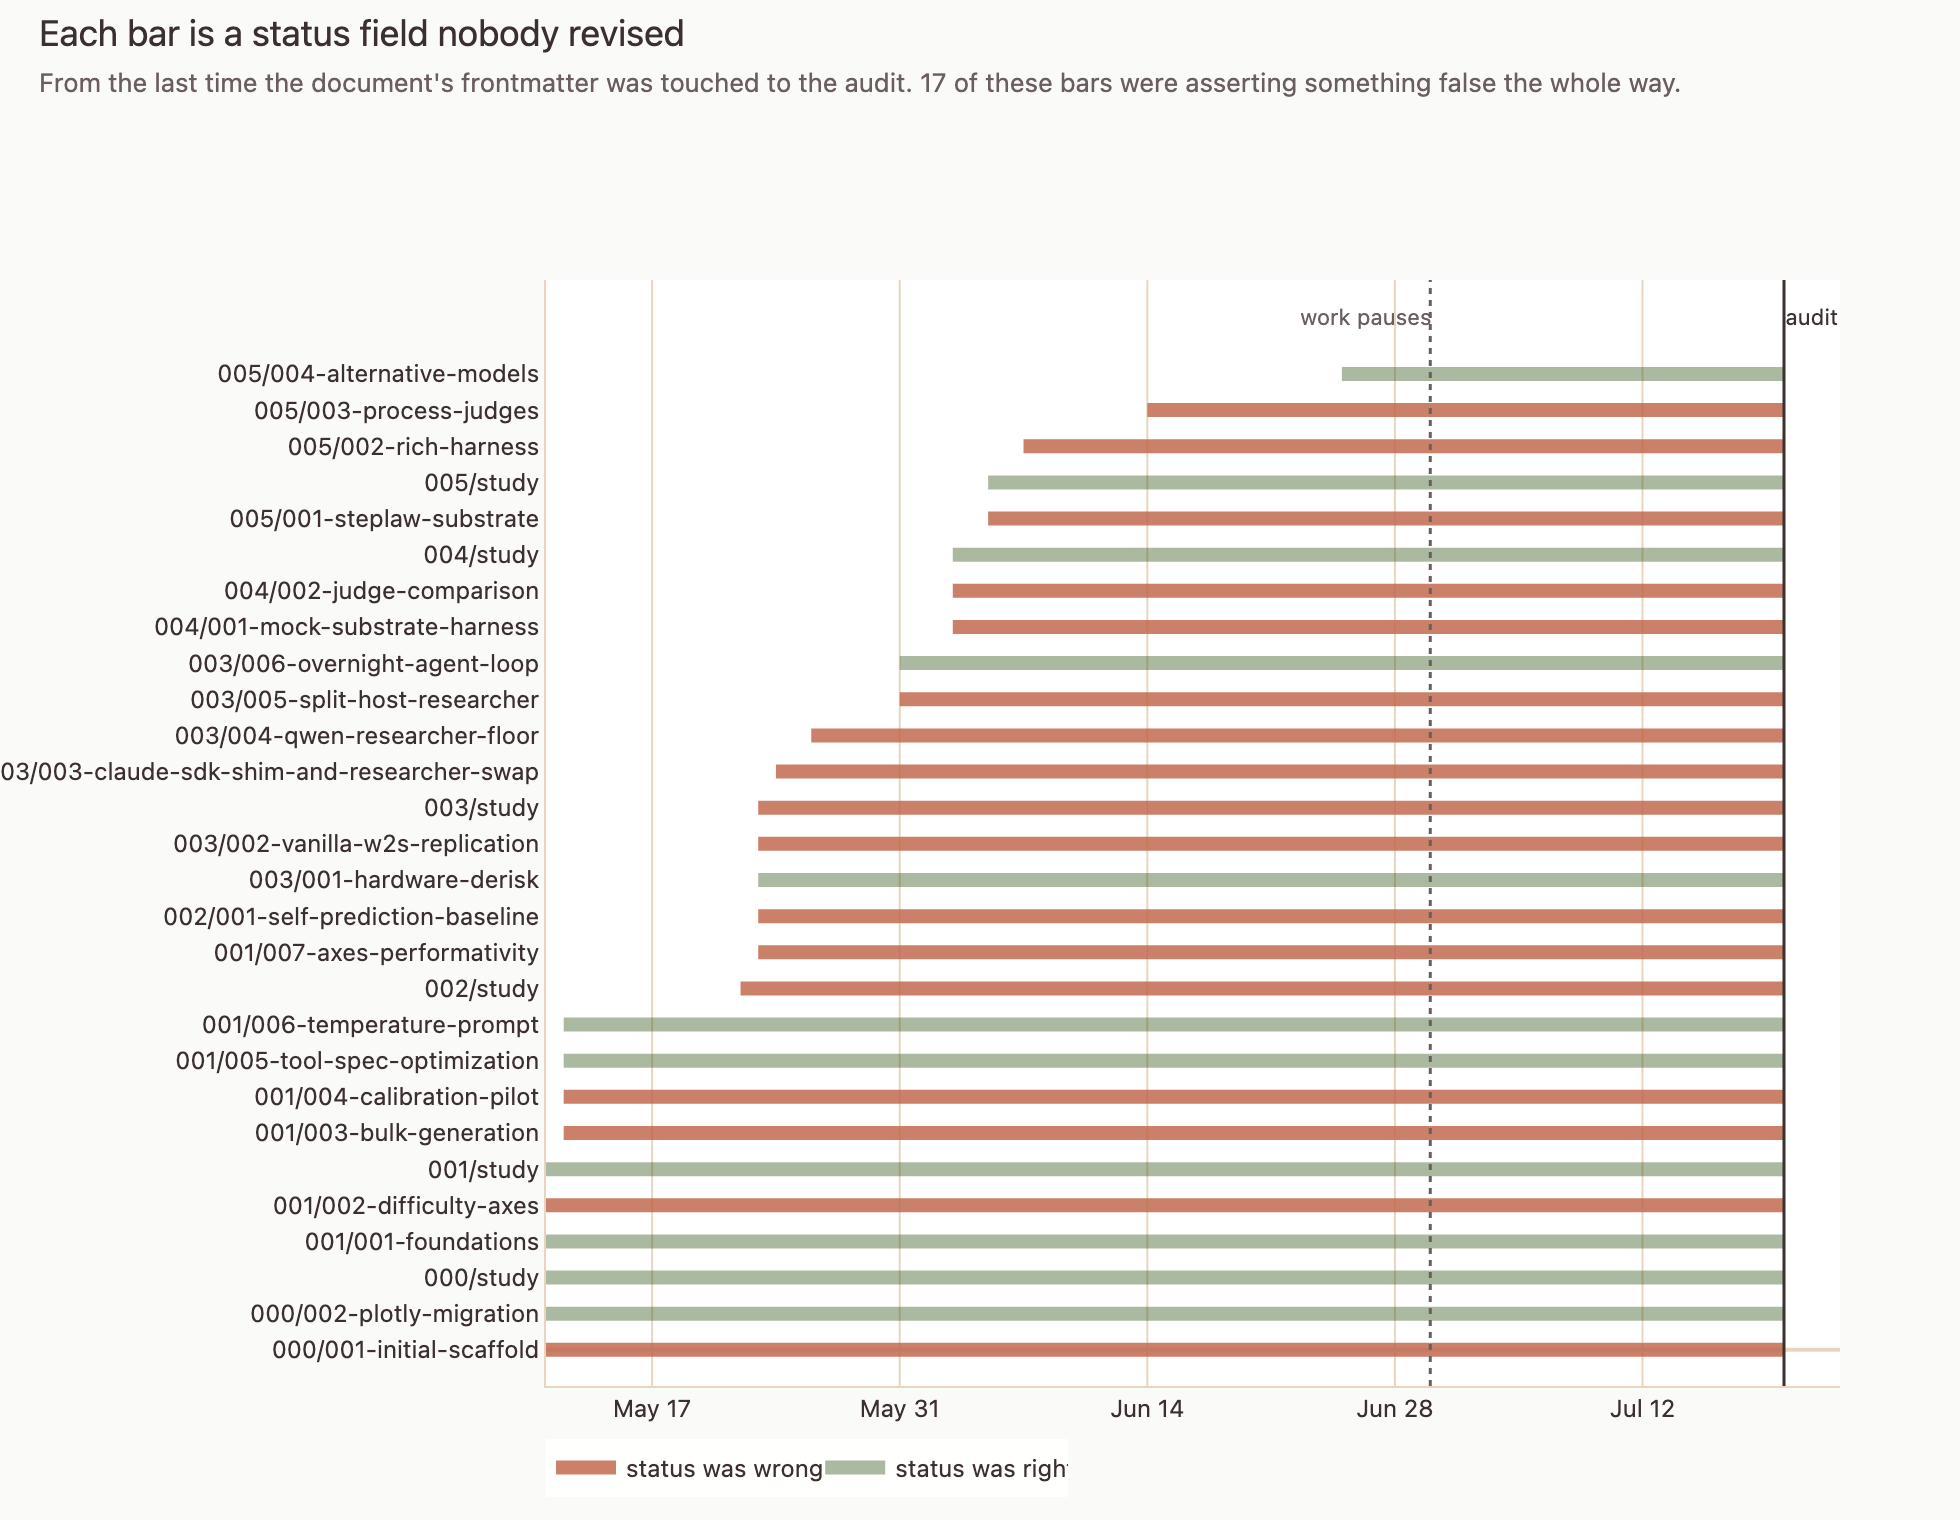
\includegraphics[width=0.88\textwidth]{figures/staleness_timeline.png}
  \caption{Each bar spans from a document's last frontmatter revision to the
  audit. Terracotta bars were asserting a false status for their entire
  length. Note that wrongness does not track age: several May documents
  stayed accurate while several June documents did not. What predicts error
  is not elapsed time but whether a successor investigation existed
  (Section~\ref{sec:mechanism}).}
  \label{fig:timeline}
\end{figure}

\subsection{Drift was not confined to the machine-readable layer}

This matters because it removes the cheap fix. If only the YAML had rotted,
a linter would resolve the problem. The prose bodies drifted independently:

\begin{itemize}[topsep=3pt,itemsep=1pt]
  \item \texttt{003/study.md} listed investigation 001 as
        ``Planned (next up)''; that child's own document reads
        ``\textbf{Verdict: GREEN}'' and is marked complete.
  \item \texttt{005/study.md} listed its investigation 003 as a task that
        investigation 003 is not, and omitted investigation 004 entirely.
  \item One investigation carries the live subheading ``Phase 2 ---
        \emph{(in progress)}'' directly above a line reading
        ``\textbf{Status:} Phase 2 complete''.
  \item One investigation has three of its closing sections duplicated
        verbatim.
\end{itemize}

\noindent
Three layers --- frontmatter, derived index, and prose --- disagreed with
each other and with the data on disk.

\subsection{The taxonomy could not express the shape of the work}

A second, structurally distinct failure. The schema assumes work nests:
study contains investigation. Real work crossed those boundaries
constantly, and the frontmatter had no vocabulary for it. The
\texttt{related} field exists but is untyped, so it cannot distinguish
``superseded by,'' ``absorbed the remainder of,'' ``failed into,'' or
``see also.'' Concrete instances found during reconciliation:

\begin{itemize}[topsep=3pt,itemsep=1pt]
  \item An investigation under study 004 finished its own question, but its
        stated follow-on was executed by an investigation under
        \emph{study 005}. No status value can encode ``complete, because a
        sibling under a different parent absorbed the remainder'' --- which
        is exactly why the document read as ambiguous to a fresh reader.
  \item An investigation under study 001 pivoted mid-flight and handed its
        reformulation to study 002, which did not yet exist.
  \item Three consecutive investigations in study 003 form a chain in which
        each link's \emph{failure} is the next link's scope.
\end{itemize}

\noindent
The lineage graph was a DAG with typed edges. The schema recorded a tree
with untyped ones. This also explains a downstream complaint --- that
rendering the lineage graph proved awkward --- as a consequence rather than
a separate problem: one cannot draw edges that were never recorded.

Note the asymmetry. In all seven documents whose state was undecidable from
frontmatter, the \emph{prose} handoff to a named successor was accurate.
The information existed; the schema had nowhere to put it.

\section{Mechanism: byproduct versus bookkeeping}
\label{sec:mechanism}

Sorting the artifacts by whether they survived produces a clean partition.

\begin{table}[h]
\centering
\small
\begin{tabular}{@{}p{0.46\textwidth}p{0.46\textwidth}@{}}
\toprule
\textbf{Held true} & \textbf{Went stale} \\
\midrule
Dated log entries inside investigations &
  Frontmatter \texttt{status} \\
Numeric results and result tables &
  Frontmatter \texttt{updated} \\
Rendered run and trace reports &
  The derived \texttt{lineage.yaml} \\
Pre-registered stopping criteria &
  The ``Investigations'' lists inside \texttt{study.md} \\
\texttt{HANDOFF.md} (see below) & \\
\bottomrule
\end{tabular}
\end{table}

\noindent
Every surviving item was generated \emph{because the researcher wanted it
for its own sake at the moment of writing}. You add a result because you
have a result. You write a log entry because something happened. Every
failed item required a separate act performed for the benefit of a future
reader.

Status is the extreme case of the second category, and structurally so:
\textbf{it is the one field that must be written at a moment when there is
no reason to write it.} Closing out a status happens after the interesting
part is over --- and, characteristically, at the same moment a successor
investigation is becoming interesting. All five \texttt{planned}-but-done
documents are cases where a successor existed. The researcher's attention
had already moved to the child.

\subsection{The exception that supports the mechanism}

\texttt{HANDOFF.md} is a pure bookkeeping artifact --- written entirely for
a future reader, coupled to no result --- and it was accurate. It was
written once, under real pressure (an agent session approaching context
exhaustion, handing off to a successor), rather than maintained
continuously. This is consistent with the mechanism if the operative
variable is \emph{maintenance} rather than \emph{purpose}: a bookkeeping
artifact written once at a moment when it is load-bearing behaves like a
byproduct. We did not verify whether it was ever revised, so this reading is
under-determined by the evidence.

\subsection{The counterexample that sharpens it}

Investigation \texttt{003/004} pre-registered a stopping rule with an
explicit either-way clause: iterate until the agent completes one valid
end-to-end submission, \emph{or} until five distinct patches have been tried
without progress --- ``either outcome is the result.''

It stopped at patch 4, on protocol, and said so in the document while the
work was live: a fifth patch ``would only re-test prompt variants on the
same broken substrate.'' It handed forward a sharp, correct diagnosis.

Same document, same author, same week: the pre-registered budget was
consulted and obeyed; the \texttt{status} field went stale. The difference
is not discipline. It is whether the field had a job to do \emph{during} the
work or only after it.

\section{Why this is worse than no index}

The framework's goal was to make state legible to a fresh agent. It instead
produced state that was \emph{plausibly formatted and wrong}.

An empty field prompts a question. A stale field suppresses one. A fresh
reader --- human or agent --- who consults \texttt{lineage.yaml} and reads
\texttt{status: planned} on a study containing a 4{,}392-call experiment
does not go looking; the index has already answered. We can confirm this is
not hypothetical: the derived index was verified to carry
\texttt{status: planned} for four documents that had run and analyzed
experiments, and the session that discovered the drift did so only because
it had been asked to audit, not because the index looked suspicious.

The second-order cost is the more expensive one. Seven documents (25\%) had
a state that was \emph{undecidable from the text} at audit time. By the time
anyone reconciled, the information needed to close them out no longer
existed in the artifacts and had to be reconstructed from the researcher's
memory --- a resource that does not survive a five-week absence intact and
does not exist at all for a fresh agent.

\section{Why ``just be more disciplined'' is not available}

The repository's own first investigation predicted this failure, in writing,
on day one, in its Limitations section: ``No CI / hooks wired up --- humans
must remember to run \texttt{update\_lineage.py} \ldots after edits.'' It
listed the fix among its follow-ons: a frontmatter validator, and a
pre-commit hook.

A pre-commit hook exists on disk. No frontmatter validator does. The
mechanism that would have caught the drift was scoped, written down, and
never built --- while the ceremony it was meant to protect was performed 28
times.

And that first investigation is itself an instance of the failure. Every
artifact it set out to build was delivered and the work finished; it simply
was never marked \texttt{complete}. It sat at \texttt{in-progress} from
2026-05-11 until 2026-07-20, closed out only during this reconciliation. The
investigation that \emph{created} the status convention, and that
\emph{predicted in writing} the failure to maintain it, was the first
document to exhibit it.

\section{What the framework did buy}
\label{sec:bought}

A report that only indicts is not credible, and the framework returned real
value along its non-bookkeeping dimensions.

\begin{itemize}[topsep=3pt,itemsep=1pt]
  \item \textbf{The investigation boundary worked as a stopping device.} The
        pre-registered patch budget in Section~\ref{sec:mechanism} fired as
        designed and prevented a tar-pit.
  \item \textbf{Pre-registered hypotheses let negative results be reported
        as results.} A component registry with hypotheses scored in advance
        is why a 120-run factorial that mostly disconfirmed its own
        predictions reads as a finding rather than a failure.
  \item \textbf{Successor handoffs were traceable.} Every one of the seven
        undecidable documents named its successor, and every pointer was
        correct. The lineage was right about \emph{shape} even where it was
        wrong about \emph{state}.
\end{itemize}

\noindent
The framework's value, in other words, concentrated in exactly the places
where a field had a job during the work. That is the same seam.

\section{Design implications}

These follow from the mechanism; none has been tried, and the third is
speculative.

\begin{enumerate}[topsep=3pt,itemsep=2pt]
  \item \textbf{Couple bookkeeping to an act already being performed.} Make
        status a by-product: an investigation cannot record results without
        declaring whether its stopping criterion was met. The pre-registered
        budget survived precisely because it was consulted mid-work.
  \item \textbf{Automate the check, and fail loudly.} A hook that
        regenerates the index, and --- more importantly --- \emph{fails}
        when a document's \texttt{updated} predates its own newest dated
        content, or when a \texttt{planned} document contains a Results
        section. This exact mechanism was named on day one and never built,
        so a proposal to build it now owes an account of why the second
        attempt sticks where the first did not. The honest answer is
        probably that it must be enforced by something other than intent.
  \item \textbf{Prefer new primitives to new discipline.} Make a parent's
        state a \emph{computed function} of its children rather than a
        hand-maintained claim --- which would have prevented all five
        \texttt{planned}-but-done cases --- and let the return value carry
        typed edges, addressing the DAG problem in the same move.
\end{enumerate}

\noindent
There is a strategic fork underneath all three. Options 1 and 3 want control
over the agent loop itself: ``you may not write results without closing
status'' is a harness-level constraint, and conventions written in an
instructions file are exactly the optional bookkeeping that failed here. The
counter-argument is that a custom harness is a large build with unknown
failure modes. Unresolved.

\section{Limitations}
\label{sec:limits}

\begin{itemize}[topsep=3pt,itemsep=1pt]
  \item \textbf{Ground truth is not independent.} The reconciled status
        against which drift is measured was assigned by the same researcher
        whose bookkeeping is under audit, assisted by a language model. The
        five \texttt{planned}-but-done cases are unambiguous; the softer
        twelve involve judgment about when analysis becomes ``complete.''
  \item \textbf{An earlier internal audit undercounted.} A prior pass
        reported 13 mismatches (46\%); full reconciliation produced 17
        (61\%), and the 46\% figure coincides exactly with a different
        measure (stale \texttt{updated} dates). An audit performed by a
        language model reading documents is itself an instrument with error,
        and this one erred toward under-reporting.
  \item \textbf{$n=28$ documents, one repository, one researcher,} with an
        unusual work pattern (intense bursts separated by a five-week
        absence). Whether the byproduct/bookkeeping split generalizes to
        teams, or to repositories with review gates, is untested.
  \item \textbf{The mechanism was named after seeing the data.} The
        byproduct-versus-bookkeeping partition fits all 28 cases, but the
        categories were chosen with the outcomes visible. It is a hypothesis
        that the data does not contradict, not a result. It is testable: a
        second repository with the same conventions, audited blind, should
        show the same partition.
\end{itemize}

\section{Conclusion}

A metadata system designed to make research legible to a fresh agent
produced, after twelve weeks, an index that was confidently wrong about 61\%
of its corpus and had never once erred toward understating progress. The
failure was not technical and was not, in any useful sense, a failure of
discipline: the fields that survived and the fields that rotted are cleanly
separated by whether maintaining them was coupled to work the researcher had
independent reason to do. The design implication is not a better convention.
Conventions are the thing that failed. It is to move status out of the
category of things one remembers, and into the category of things one cannot
avoid producing.

\vfill
\noindent\rule{\textwidth}{0.4pt}\\
\footnotesize
Source evidence pack:
\texttt{studies/000-research-organization/framework-drift-evidence.md}.
Snapshot: \texttt{drift-snapshot.tsv}. Figures regenerate via
\texttt{writeups/technical-reports/framework-drift/figures/}. Repository
state pinned at tag \texttt{framework-v1}.

\end{document}
